% Chapter Name
\chapter{\sc A Low Energy Electron Microscopy Investigation of Polymorphic Graphene}
\label{ch:A Low Energy Electron Microscopy Investigation of Polymorphic Graphene}

\section{Preliminary LEEM investigation of polymorphic graphene}
In order to more fully characterize the polymorphic graphene system, further surface science tools beyond conventional LEED, AES, and STM are required. In collaboration with the Center for Integrate Nano-Technology, CINT, at Sandia National Laboratory in Albuquerque, NM, a preliminary study of the polymorphic graphene system has been conducted using a low energy electron microscope. To begin this study, a polymorphic graphene sample was prepared at UNH using the method outlined in Chapter 4.

A small section of the sample surface area was found to display the characteristic conventional LEED signature of polymorphic graphene. Minimal other characterization was performed at UNH before packaging the sample for transit. The sample was transported to Sandia while still mounted within its UHV sample holder, however an additional solid washer was installed above the sample surface to prevent contact to the sample surface during transit.

Upon arrival at the CINT facility at Sandia, the sample holder assembly was disassembled so the ruthenium crystal could be mounted on the LEEM system sample holder. During this step it was crucial to keep track of sample orientation so that a specific area on the sample could be found during LEEM analysis. At this point it was noted that the ruthenium crystal had a distinct crack and warp on one section of the crystal, which made for an easy reference point, however this sample feature would have other important implications later in the study. Since the sample was transported to Sandia in air, it was necessary to perform a significant outgassing step under high vacuum before a LEEM investigation could be started. During this phase the sample was heated to 200$^{\circ}$ C by a rear mounted filament and allowed to outgas for some few hours. The pressure in the preparation chamber rose to over $10^{-8}$ torr at this point, indicating a high amount of outgassing from the sample.

\begin{figure}
  \centering
  \includegraphics[scale=0.75]{./figs/LEEM-islands.jpg}
  \caption{
  Real Space 50 $\mu$m FOV LEEM image of the graphene/ruthenium system displaying characteristic lens shaped graphene islands, which appear as darker islands atop a brighter background. Image collected with incident beam energy of 13.9 eV. Data shown is part of a LEEM-\textit{I(V)} data set collected with 0.1 eV energy steps between images. Most islands are 3-5 $\mu$m at max width.
  }
  \label{fig:LEEM-islands}
\end{figure}

Upon initial investigation with real space LEEM using a 50 $\mu$m FOV, areas of the sample containing lens shaped islands were readily visible. These areas were identified as graphene islands and matched well with other reported studies of the graphene/ruthenium system using LEEM \cite{sutterleem}. Knowing the FOV of the LEEM images was 50 $\mu$m, the size of the graphene islands could be estimated to be multiple microns at their widest points. Here the relative coverage of graphene on the Ru(0001) surface can be estimated quickly due to the fast imaging nature of LEEM. The experiment demonstrated that samples could be grown ex-situ and transported to Sandia for imaging with minimal preparation needed before data collection.

\begin{figure}
  \subfloat[Real space LEEM image at 0.5eV incident energy with 50 micron FOV \label{subfig1}]{
    \includegraphics[scale=0.5]{./figs/mLEED1.png}
  }
  \hfill
  \subfloat[Aperture limited real space LEEM image \label{subfig2}]{
    \includegraphics[scale=0.5]{./figs/mLEED2.png}
  }
  \\
  \subfloat[Overlay of (a) and (b) with 40\% transparency showing which part of the sample is imaged to acquire the data shown in (d) \label{subfig3}]{
    \includegraphics[scale=0.5]{./figs/mLEED3.png}
  }
  \hfill
  \subfloat[$\mu$-LEED image from roughly 5 micron illuminated section of sample. Reciprocal space image acquired at 50.0 eV. Ru (1x1) peaks are visible along with carbon satellite peaks typical of the graphene/ruthenium system.
                \label{subfig4}]{
    \includegraphics[scale=0.5]{./figs/mLEED4.png}
  }
  \caption{
  The $\mu$-LEED process shown where a specific location on the sample can be selected for acquisition of reciprocal space data. This process is sometimes referred to as selected area low energy electron diffraction.
  }
  \label{fig:microleed}
 \end{figure}

Further investigation of the sample at Sandia using $\mu$-LEED imaging was carried out in sample regions with visible graphene islands. The $\mu$-LEED technique allowed for a very high degree of control concerning which areas of the sample were imaged in reciprocal space by using micron sized apertures. To do so a large area real space LEEM image was acquired first so that areas of interest could be located. In this investigation we sought to image the graphene islands as well as the surrounding area with reciprocal space mapping. At this point a beam-limiting aperture was positioned in the beam line of the reflected electron beam after exiting the objective lens system before entering the transfer lens to the imaging column. This restricted the acquired image of the electron beam spot to a fixed diameter. With the aperture in place, a second real space image was collected such that only data from within the beam spot was acquired. By overlaying both real space images atop one another using post-processing software, the exact spot on the sample can be seen where reciprocal space data was collected.

Using the above technique, $\mu$-LEED patterns were collected from graphene islands as well as the surface between the islands. The LEED data was collected using a 5 $\mu$m aperture. Thus data was collected from an area on the sample illuminated by an approximately circular electron beam spot with roughly five micron diameter. Figure \ref{fig:microleed} shows an example of a real space LEEM image with graphene islands, an aperture limited real space image, the overlay of the two images together, and finally the LEED pattern acquired at a fixed energy from the spot illuminated in the images. The observed $\mu$-LEED patterns do not show evidence of extra diffraction peaks as were observed using conventional LEED at UNH. This is likely attributed to the limited area on the sample that was discovered to display polymorphic characteristics when characterized at UNH. Due to time restrictions and further experimental complications, the exact position of the sample that displayed polymorphic signatures could not be located.

\begin{figure}
  \centering
  \includegraphics[scale=0.55]{./figs/IVDiagram.png}
   \caption{
  Example of a LEEM-\textit{I(V)} data set. A sequence of 250 real space images (left) are stacked vertically according to the incident electron energy at which the image was acquired. The energy step between images is 0.1 eV. \textit{I(V)} curves (right) are extracted by selecting the pixel intensity from a single pixel (highlighted in red) in each image sliced vertically through the energy axis. The structure of the curves relates to the three-dimensional structure of the sample material.
  }
  \label{fig:LEEM-I(V)-Example}
\end{figure}

Aside from the $\mu$-LEED patterns collected from the sample, a second data set using real space images was collected to allow for intensity-voltage (LEEM-\textit{I(V)}) analysis of the graphene/ruthenium system at very low incident energy. Specifically, this type of data set was of interest to look for a signature of carbon layer thickness. With STM analysis, measuring the exact layer thickness is difficult and slow. Due to the rapid imaging nature of LEEM, there is potential to quickly determine the layer thickness of many locations on the sample surface by analyzing oscillations in the electron reflectivity curves collected from many small regions.


LEEM-\textit{I(V)} data sets can be envisioned as a vertical stack of multiple real-space LEEM images from the same location on the sample captured at various incident electron energies. The LEEM control software automates the procedure such that images are captured at the same location with a fixed energy step in-between consecutive images. For LEEM-\textit{I(V)}, the step energy between images can be as low as 0.1eV. Thus covering an energy range of 0-15 eV, a LEEM-\textit{I(V)} data set with a step energy of 0.1eV consists of 150 images stacked vertically such that the vertical axis maps directly to the incident electron energy. An example of this is shown in figure \ref{fig:LEEM-I(V)-Example}. PLEASE, the Python Low-energy Electron Analysis SuitE, is the custom designed software package used for processing and analysis of LEEM and LEED data sets from graphene and other 2D materials. More details about the software can be found in Appendix A.

Previous experiments have demonstrated that oscillations in LEEM-\textit{I(V)} curves from graphene on silicone carbide correlate well to the number of carbon layers in the system as a result of thin film interference \cite{hibino-prb-g-sic}. This interference effect can be explained by the presence of quantum well states in the system; when an electron is incident on the thin film with an energy corresponding to a quantized energy state in the conduction band, then the electron will undergo resonant transmission through the film \cite{hibino-prb-g-sic, QSE}.  Transmission through the film in this manner results in a lower observed electron reflectivity. Thus by recording the electron reflectivity as a function of energy, which is effectively an \textit{I(V)} curve, the thickness of the film can be determined by analyzing the minima in the reflectivity curve. Similar modulations of the electron reflectivity spectrum have been observed in the graphene on ruthenium system \cite{sutterleem}. Thus, it is expected that the same method may be effective for analysis of the polymorphic graphene system.

Figure \ref{fig:LEEM-I(V)-Example} shows a typical LEEM-\textit{I(V)} curve extracted from the data collected at Sandia. The energy shown along the X axis is the difference between the electron source energy and the bias applied to the sample at the cathode. Thus, the initial data points have a negative energy indicative of the mirror-electron mode. Here the incident electrons have lower energy than the cathode lens and thus do not penetrate the sample surface but instead interact only weakly with the surface potential before being repelled back to the imaging column. All electrons are reflected in this mode, thus the observed intensity is very large. When the energy increases above the mirror electron threshold, the incident electrons begin to interact with the sample and the observed intensity has a drastic drop off. After this drop off two prominent oscillations are seen near 1 eV and 4 eV. These two minima may suggest that the carbon film in this region consists of two layers. LEEM-\textit{I(V)} curves with two minima represent the majority of observed curves, however, some locations display curves with other shapes as shown in Figure \ref{fig:LEEM-curves}. Also, many locations in the real space LEEM are observed to have similar \textit{I(V)} curve characteristics both on and off the areas identified as graphene islands. This complicates the direct attribution of number of minima to number of carbon layers.

\begin{figure}
  \centering
  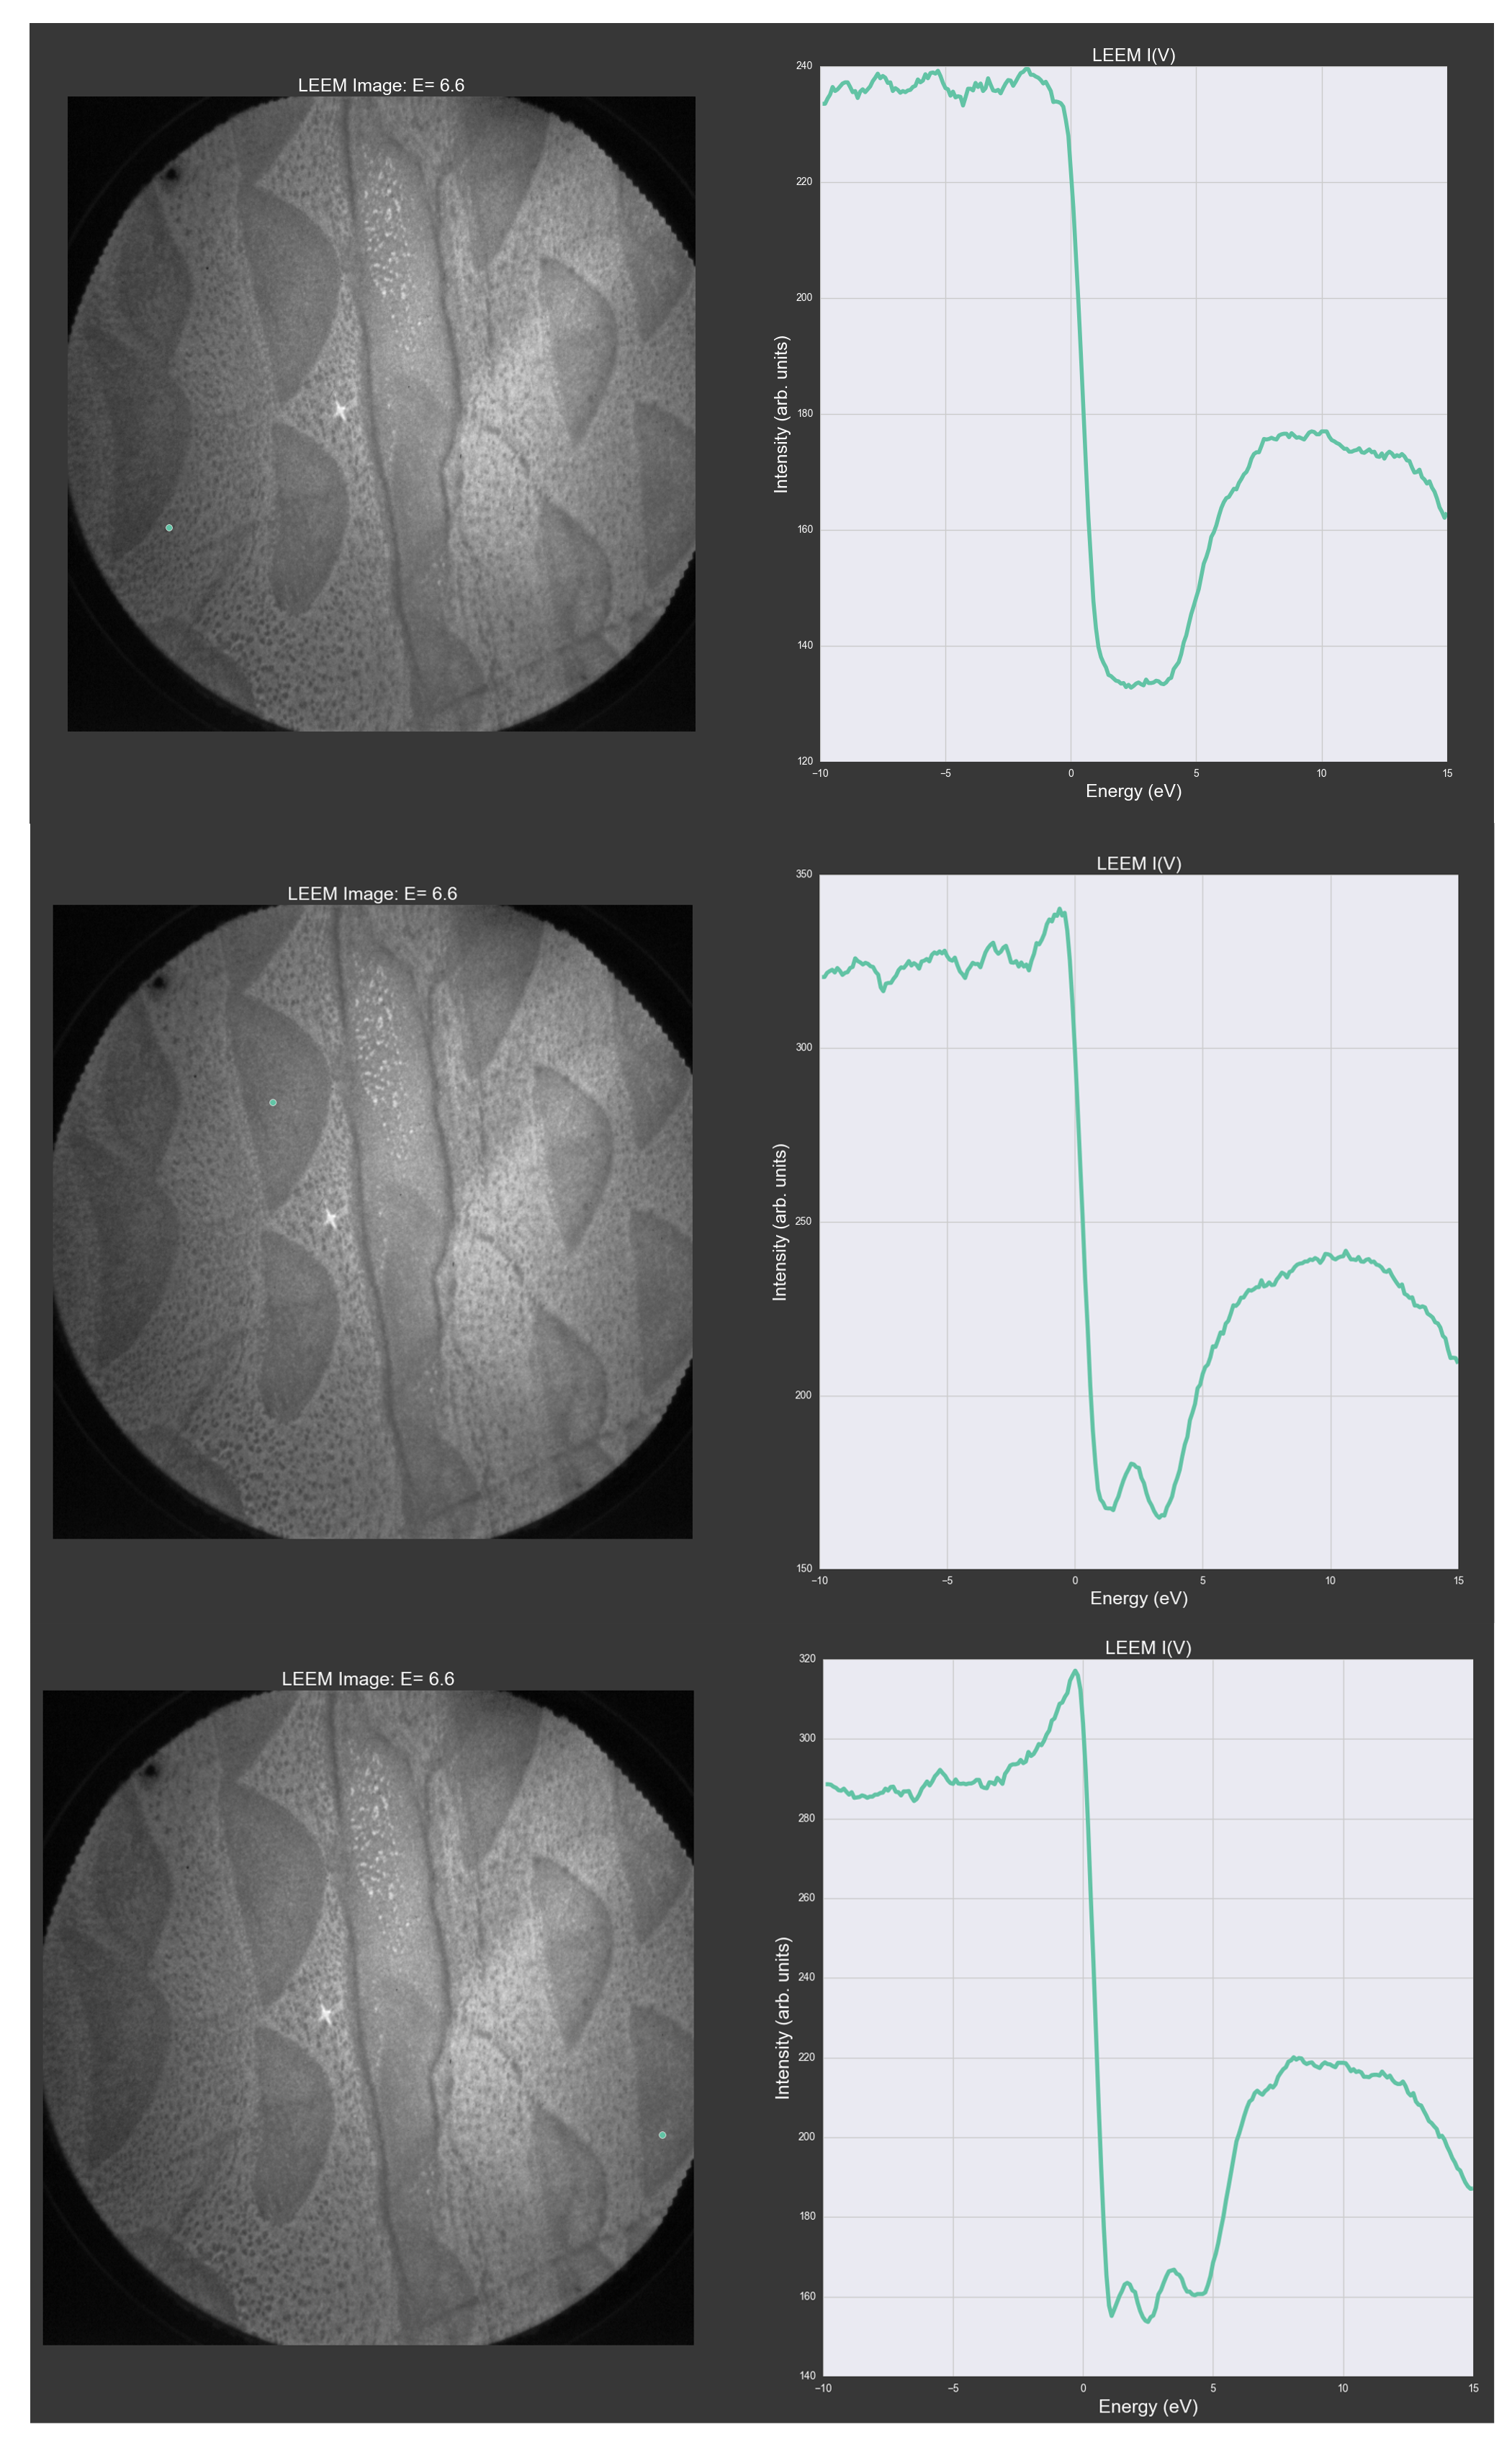
\includegraphics[scale=0.18]{./figs/threeplots.png}
  \caption{Example of different LEEM-\textit{I(V)} curve shapes observed in initial study of the graphene/ruthenium system. Real space images acquired at 6.6eV; Data extraction location marked with green dots in the left hand side real space images.}
  \label{fig:LEEM-curves}
\end{figure}

Further complicating the analysis, Figure \ref{fig:2dips-2locations} compares the \textit{I(V)} data extracted from two different areas on the sample surface which both exhibit similar \textit{I(V)} shapes. If the large dark islands are believed to be graphene islands surrounded by a lighter area consisting of ruthenium, then one would expect the two areas to have different \textit{I(V)} characteristics. One possibility is that the lighter area between the islands is actually the ruthenium surface covered by amorphous carbon which has yet to form into an ordered graphene island. If this is indeed the case then its possible that some areas of the amorphous carbon are more ordered than others and are just beginning to form graphene islands. These areas then would be expected to appear the same as what is seen from the darker island regions. While this explains why two regions may share similar \textit{I(V)} characteristics, it does not explain why two minima are observed in the \textit{I(V)} curve. If the island represents two carbon layers then the interior region between islands should show a signal of being just one layer with a single minima. Its also possible that the mapping between minima and number of layers should instead be N minima mapping to N-1 layers. This would indicate that the island regions are then single layer graphene. However, this is not the case presented by a previous study of the graphene/ruthenium system \cite{sutterleem}.


\begin{figure}
  \centering
  \includegraphics[scale=0.23]{./figs/2dips-2locations.png}
  \caption{LEEM-\textit{I(V)} extracted from two different sample areas displaying similar \textit{I(V)} characteristics. The green curve comes from an area believed to be a graphene island, the orange area would be suspected to be bare ruthenium or ruthenium with amorphous carbon.}
  \label{fig:2dips-2locations}
\end{figure}

Finally, since little STM data was recorded prior to the LEEM investigation of this sample, bilayer graphene can not be fully ruled out as a possibility for the surface structure in this sample. Whereas graphene growth by CVD on ruthenium is a self terminating process resulting in only a single layer, growth by segregation and PVD has the potential to grow multiple layers. Thus, given the inconsistencies present in the LEEM-\textit{I(V)} data extracted from our sample, no definite conclusion can be drawn concerning the sample's carbon layer thickness. However, the data collected during this experiment was still useful. Analysis of the LEEM/LEED images and LEEM-\textit{I(V)} data sets collected laid the groundwork for the PLEASE software package, which is still under active development, and is being used for further studies of numerous 2D materials beyond graphene.

Further data was prohibited as a result of a spark in the electron optics during the third day of analysis. The spark happened near the objective lens, thus the most likely culprit was the sample surface being warped. As mentioned previously, the ruthenium substrate was not uniform and had a pronounced warp/crack on one edge. This part of the sample was then closer to the objective lens than the rest of the sample surface. Given that operation of LEEM requires a very high electric field between the sample surface and objective lens, a rough sample has a tendency to create sparks. After the spark, alignment of the beam became very troublesome.

The final data set collected consisted of a random walk in reciprocal space. The beam alignment made quantitative measurements from the reciprocal space images impossible due to asymmetry in the observed patterns. Walking across the sample and observing the reciprocal space pattern showed mostly LEED signatures from Ruthenium and Graphene. However, one location on the sample was found that contained a very large number of extra diffraction spots in a variety of patterns. The pattern asymmetry makes analysis of the exact periodicity difficult, however, the patterns are still relatively well defined, as shown in Figure \ref{fig:ExtraLEEDSpots}. The cause of these extra peaks can not be confirmed; the spark may have sputtered various metals or other residual gas elements onto the sample surface. The observed patterns do not correspond to the $(2\sqrt{3}$ x $2\sqrt{3})$R30$^\circ$ previously observed via conventional LEED on the polymorphic sample, however, the beam spot size used to acquire this image is more than an order of magnitude smaller than what is possible using conventional LEED at UNH. No definitive conclusions can be drawn from this data concerning evidence of polymorphism.

\begin{figure}
  \centering
  \includegraphics[scale=0.5]{./figs/extraLEED}
  \caption{An area of the sample was observed in reciprocal space which contained many extra diffraction spots relative to the primary ruthenium (1x1) pattern and the carbon moire peaks. Due to beam asymmetry as result of a spark in the electron optics, no quantitative measurements could be performed, nor could a real space image be brought into focus at this point in the sample.}
  \label{fig:ExtraLEEDSpots}
\end{figure}

\section{Results from first LEEM experiment}

Though we were unable to obtain the data concerning the sample surface structure and the carbon layer thickness, the initial experiment was not a total failure. First and foremost, the direct outcome of this experiment was the development of the PLEASE software package for LEEM and LEED data analysis. Chapter 6 will detail further uses of this software with respect to more quantitive analysis of material surface structure. Also, a direct result of this experiment was insight into the difficulties pertaining to data analysis of the polymorphic graphene system's \textit{I(V)} characteristics without a suitable guide for the characteristics for a known structure. To address some of these issues, a second LEEM/LEED experiment focused on furthering our understanding of the growth process was carried out at the Center for Functional Nanomaterials at Brookhaven National Laboratory.


\section{LEEM investigation on the influence of hydrogen in the graphene growth process}
While the first LEEM investigation of polymorphic graphene relied on studying the sample post growth after transit to the LEEM system, our second experiment focused on studying the influence of hydrogen on the growth dynamics of graphene on ruthenium. For this experiment all graphene growth was monitored in real time through LEEM/PEEM. The experiment was carried out at the Center for Functional Nanomaterials at Brookhaven National Laboratory using the Elmitec LEEM-V system, shown in figure \ref{fig:LEEM-V}.

In order to study the effects of hydrogen on the graphene growth process, a source of atomic hydrogen was added to the main LEEM chamber. A commercial thermal gas cracking device provided a flux of atomic hydrogen with controllable pressure to the main LEEM chamber, thus allowing graphene growth to take place in a hydrogen atmosphere while simultaneously imaging the surface with LEEM or PEEM. After installation of the hydrogen cracking source, the LEEM system was baked to obtain low pressures. Next, the electron optics were realigned using a combination of Au/Si and Si(111) samples. Temperatures in the experiment were measured with a C-Type thermocouple attached behind the sample surface. The thermocouple was calibrated using a single point method by observing the silicon (7x7) to (1x1) surface phase transition with real time LEED. The known phase transition temperature of 1100K \cite{Si111} was compared to the TC temp recorded during the transition in order to calculate an offset between the measured temperature and the known temperature. Due to time constraints, only one temperature calibration point was used. Thus the temperatures in this experiment were known to within 25-50K. The difference in LEED pattern observed from the two Si(111) surfaces can be seen in figure \ref{fig:Si(111)}. Future experiments would may more accurately perform the temperature calibration by using a second surface transition at a different temperature to perform a two-point calibration.


\begin{figure}
    \centering
    \includegraphics[scale=0.13]{./figs/LEEM-V1.jpg}
    \caption{
    The Elmitec LEEM-V system at the BNL CFN features a T-shape beamline configuration: Electron source (bottom left side); Main chamber, objective lens, and hydrogen cracking source (top left); magnetic prism array (center); imaging column and CCD (right side).
    }
    \label{fig:LEEM-V}
\end{figure}


\begin{figure}
  \subfloat[(7x7) surface reconstruction of Si(111)]{
    \includegraphics[scale=0.22]{./figs/Si(111)7x7.png}
  }
  \hfill
  \subfloat[Pristine (1x1) Si(111) surface]{
    \includegraphics[scale=0.22]{./figs/Si(111)1x1.png}
  }
  \caption{
  The C-type thermocouple was calibrated by imaging the surface of Si(111) in reciprocal space and observing the temperature dependent transition from the (7x7) reconstruction [Left] to the (1x1) phase [Right], which occurs at 1100K.
  }
  \label{fig:Si(111)}
\end{figure}

To begin the sample preparation for this experiment, a Ru(0001) crystal was degassed in the preparation chamber above 400K for a few hours to remove water before being transferred to the main LEEM chamber. Preliminary imaging of the surface showed large amounts of carbon contamination and a high degree of roughness as determined by large amounts of disordered step bunches seen in LEEM. The surface was sputtered with argon ions for 30 mins followed by a standard procedure of exposure to oxygen followed by high temperature annealing to remove carbon. After repeated cycles of oxygen exposure and annealing, a clean Ru(0001) surface was obtained, as verified by a clean Ru p(1x1) LEED pattern free of any other LEED spots as well as a uniformly dark PEEM image. The ruthenium surface has a high work function and thus appears dark when imaged with PEEM, whereas carbon on the ruthenium surface present as adatoms in an amorphous phase or ordered graphene will have a very high signal in PEEM imaging mode.

\begin{figure}
        \includegraphics[scale=1.05]{./figs/LEEM-Ru-Before-After-150.png}
    \caption{Real-space LEEM images of the Ru(0001) surface slightly defocused to enhance the contrast of steps and step bunches on the surface. Steps and step bunches appear as dark marks on an otherwise bright surface. Left: 20 micron FOV image of the ruthenium surface after annealing before sputtering. Poor surface quality is indicated by frequency of step bunches and shorter disordered steps. Right: 10 micron FOV LEEM image after sputtering the surface and completing numerous cycles of flash annealing and oxygen exposure. Overall surface quality has improved.
    }
    \label{fig:LEEM-Ru-before-after}
\end{figure}



Figure \ref{fig:LEEM-Ru-before-after} shows two LEEM images of the Ru(0001) acquired before and after sputtering. The image after sputtering appeared clean enough to begin further studies. A LEED-\textit{I(V)} data set was acquired for the clean Ru(0001) surface, covering an energy range of 30-250 eV. A comparison of this data to previously reported conventional LEED-\textit{I(V)} data shows excellent agreement \cite{Ru-LEED-old}. While previous studies on the ruthenium surface structure utilized conventional LEED, our study acquired LEED data via LEEM. Thus, included in our data is the \textit{I(V)} curve for the (0,0) spectrally reflected beam, which is typically absent from conventional LEED experiments unless an off-normal angle of incidence is used. Thus, it may be worth analyzing the optimized surface structure obtained by fitting this data to dynamic electron multiple scattering models.

After analyzing the pristine ruthenium surface, the temperature parameters for graphene growth via bulk segregation were determined. The sample surface was doped with a small amount carbon via catalytic decomposition of ethylene using a CVD process. At high temperature, the $C_{2}H_{4}$ adsorbate molecules decompose into carbon adatoms and free hydrogen molecules. This process is easily visualized in real-time with PEEM due to the large difference in work function between ruthenium and carbon. Carbon adatoms and ordered graphene islands appear as bright areas atop a dark ruthenium background. Utilizing the fact that the carbon solubility in ruthenium changes as a function of temperature, the surface phase carbon was adsorbed into the bulk ruthenium crystal at a temperature above 1000$^\circ$ C which agrees with previous results \cite{mccarty-carbon}. At this point the PEEM image of the surface returned to a uniformly dark image devoid of structure indicating the surface was only ruthenium and was ready for graphene growth via segregation. Slowly cooling the sample from 1000$^\circ$ C while recording the PEEM image every few seconds provided a movie of the graphene growth process. As the ruthenium temperature cooled, the bulk carbon solubility dropped and thus the interstitial carbon atoms diffused to the surface. The initial nucleation of carbon surface atoms appeared as a small bright spot atop the dark ruthenium background. Growth continued slowly outward from the initial nucleation point in a somewhat dendritic fashion, indicating relatively poor surface quality.

Figure \ref{fig:seg-growth} shows a sequence of images from the bulk segregation growth process described above. The initial image shows a uniformly dark ruthenium surface devoid of any photoemission signal from the light source used. As the temperature of the crystal cools from temperatures above 1200 K, carbon begins to segregate from bulk to surface. This can be seen as bright spots that appear in the later images. The islands grow outwards from the initial nucleation points. The rate of growth is influenced by a number of factors such as temperature and relative bulk carbon abundance. The kinetics of the growth process are explained in detail by McCarty et al \cite{mccarty-carbon}. Depending on the initial amount of available carbon from CVD doping and the growth time, graphene islands could be grown up to tens of microns in size.

The process of growing graphene via segregation is a reversible process. After growing islands, the sample can be heated again to high temperatures (T $>$ 1600 K) to dissolve the carbon back into the crystal bulk. This was repeated numerous times to get a better understanding of the heating and cooling parameters required to grow repeatedly grow pristine graphene islands. Next, the influence of atomic hydrogen on as-grown graphene was studied. The process of CVD doping, dissolving of surface carbon, and finally growth by segregation was repeated to nucleate a large graphene island with a length dimension larger than 20 micron.

After the island was grown, it was exposed to a flux of atomic hydrogen and monitored with LEEM to look for changes in the local electron reflectivity or other signs of interaction with the hydrogen. The idea behind this study was that it may be possible for the hydrogen to intercalate at the graphene-ruthenium interface, thus lifting the carbon layer higher above the ruthenium and passivating the ruthenium surface. While monitoring the LEEM signal from the graphene surface during hydrogen exposure at a pressure of 1 x 10$^-6$ torr, little change was observed. The sample was then subject to prolonged annealing in a hydrogen atmosphere. The only difference observed over time was mild etching of the graphene island edges. Without a simultaneous residual gas analysis of the reaction, it is difficult to determine the specifics of the observed reaction. One possibility is a reaction between hydrogen (as molecular gas phase or in atomic phase) and the graphene island edge, producing a hydrocarbon of the form \ce{C_{x}H_{y}}. Another possibility is the reaction between oxygen impurities in the hydrogen atmosphere and the graphene island edge. Oxygen is known to react with carbon at the ruthenium surface to create \ce{CO} and \ce{CO_{2}} molecules. This is the primary method for cleaning a ruthenium surface to remove unwanted carbon contaminants. A previous study has shown that oxygen contamination can induce graphene etching in graphene grown by CVD on copper foils, and furthermore, this etching can be minimized or halted altogether by using ultra purified hydrogen \cite{graphene-etching}. A second study indicates that the reaction for oxygen etching on ruthenium proceeds with a relatively low activation energy \cite{graphene-etching-ru-O2}

Regardless of what chemical reaction is involved in the graphene etching process, it was noted that during a prolonged annealing in a hydrogen atmosphere, the etching process did not continue to the entirety of the graphene island. Actually, very little surface area of the island was etched away. One possible explanation of this could be a reaction terminated by ruthenium step edges.  Graphene on ruthenium tends to grow in a ``carpet-like'' fashion, where the graphene islands grow preferentially in a the downhill direction on the ruthenium terraces with little to no growth in the uphill direction. Similarly, the etching process via hydrogen atoms or other gas impurities may etch the island up to the nearest step edge in the uphill direction and then terminate. The carbon atoms at the step edge may be more strongly bound to the ruthenium surface as a result of the higher coordination number for ruthenium atoms at the step edge. This stronger binding may interrupt the etching process.

To summarize the findings for the interaction of hydrogen with as-grown graphene islands: no signs of intercalation were observed via PEEM, LEEM, and LEED. The LEED patterns observed from graphene before and after addition of the hydrogen remained unchanged indicating no structural changes in the graphene overlayer, and the LEEM images showed no observable change in electron reflectivity. To continue the experiment, we then analyzed the effects of graphene growth on ruthenium in a hydrogen atmosphere rather than observing the effect of hydrogen on an already grown graphene island.


\begin{figure}
  \subfloat[t = 0s]{
    \includegraphics[scale=0.22]{./figs/PEEM-73.png}
  }
  \hfill
  \subfloat[t = 10s]{
    \includegraphics[scale=0.22]{./figs/PEEM-75.png}
  }
  \\
  \subfloat[t = 60s]{
    \includegraphics[scale=0.22]{./figs/PEEM-85.png}
  }
  \hfill
  \subfloat[t = 120s]{
    \includegraphics[scale=0.22]{./figs/PEEM-104.png}
  }
  \caption{Time sequence of PEEM images detailing growth of graphene islands via bulk segregation of interstitial carbon atoms from a Ru(0001) crystal. Field of View in all images is 30 micron; all times are approximate to within a few seconds, and the growth temperature is approximately 1075 K. The dark background is the ruthenium surface, devoid of any photoemission signal, as shown in panel a. The bright spots in later images indicate carbon islands that grow outward from the initial nucleation points shown in panel b.
  }
  \label{fig:seg-growth}
  \end{figure}

 To study the effect of hydrogen on the growth process of graphene on ruthenium, first the sample was pre-doped with carbon via CVD of ethylene at high temperature. Next, the surface carbon was adsorbed into bulk by high temperature annealing. The process was monitored in real time via PEEM. When the PEEM surface image became nearly uniformly dark, indicating no surface carbon. Finally, before regrowing graphene, the LEEM main chamber was backfilled with atomic hydrogen at a pressure of $10^{-6}$ torr. The process of carbon adsorption into bulk was then reversed by slowly cooling the sample from above 1000 $^\circ$ C. The growth of graphene islands via bulk segregation in a hydrogen atmosphere was monitored with LEEM and the process was continued until multiple large area islands had nucleated. Figure \ref{fig:three-islands} shows a 30 micron FOV image of three graphene islands after growth in a hydrogen atmosphere. Using the LEEM control software, three areas in the island centers were marked for analysis with LEED.

 Next the LEED patterns acquired from each island were observed by placing a 5 micron beam limiting aperture inline with the reflected/diffracted beam signals in the imaging column of the microscope and then aligning the data acquisition area with one of the previously marked locations. At each island, LEED-\textit{I(V)} data was also collected. Neither island displayed different characteristics in the observed LEED pattern compared to that of graphene grown via segregation without hydrogen. The $2\sqrt{3}$ x $2\sqrt{3}$R30$^\circ$ pattern observed after growth of polymorphic graphene at UNH was not observed after any combination of during-growth or post-growth hydrogen exposure. One possible explanation of the lack of signal of hydrogen interaction could be that the distance between hydrogen cracking device and the sample/objective lens system was too large. Given that the cracking device had to be integrated with the main LEEM chamber to to real time monitoring of the growth process, the distance to the hydrogen cracker could not be adjusted. If the mean free path of the atomic hydrogen atoms was too short, then a sufficient flux of atomic hydrogen would not reach the surface before recombination. A partial solution to this issue will be addressed later as a future experiment.

 Graphene samples were prepared using a variety of growth techniques. the CVD growth process using ethylene was the quickest way to achieve essentially a full monolayer of graphene due to the catalytic decomposition process being self terminating. However, the graphene grown by CVD was generally of poor quality, which could be seen in two ways. First, by monitoring the growth in real time it was observed that the CVD growth process proceeded from a very large number of nucleation points. Graphene would grown outward from each nucleation point resulting in a very large number of small graphene islands. As the monolayer grew to completion, the small graphene islands grew and merged together, however the domain boundaries between the individual islands did not fully go away. When observing the LEED pattern from CVD graphene it was evident that there was a very large degree of rotational disorder, likely resulting from the domain edges. It may be possible to recover a better LEED signature by a prolonged annealing of the CVD graphene sample, however this was not tested.

Graphene grown via bulk segregation generally resulted in higher quality graphene samples as characterized by LEED, however this comes with a number of downsides. The process of growth by segregation is very dependent on the initial conditions of carbon concentration in the bulk and near surface region of the ruthenium crystal. Growth will only continue while there is sufficient diffusion of interstitial carbon atoms through the bulk to the surface, thus the size of the graphene layer grown is limited by the carbon concentration. In contrast to the CVD growth process, bulk segregation is not a self terminating growth process. If there is sufficient carbon concentration in the bulk region, then multiple graphene layers can be grown. The second layer will not begin to grown until the surface has achieved approximately 0.80ML coverage, and will grow from below the first layer. \cite{sutterleem, Graphene-on-metals}

 \begin{figure}
     \centering
     \includegraphics[scale=1.1]{./figs/LEEM-three-islands-with-H.png}
     \caption{30 micron FOV displaying three large area graphene islands grown via bulk segregation of carbon in a hydrogen atmosphere. To look for indications of structural changes resulting from hydrogen interaction, each island was examined using LEED.
     }
     \label{fig:three-islands}
\end{figure}

After analyzing the growth of graphene on ruthenium under a hydrogen atmosphere using a variety of growth parameters, no LEED signatures of hydrogen influence were observed. This prevented further analysis of the surface structure parameters via LEED-\textit{I(V)} of the polymorphic graphene system. However, a number of brightfield LEEM-\textit{I(V)} data sets were collected to analyze the carbon layer thickness in the sample. First, the sample was cleaned using the previously mentioned method of cycles of high temperature annealing and oxygen exposure. Once the ruthenium surface was deemed essentially free of carbon by analyzing PEEM images and the $\mu$-LEED pattern, a brightfield LEEM-\textit{I(V)} data set was acquired for the pristine Ru(0001) surface.

Next, graphene was grown via bulk segregation in a hydrogen atmosphere until large single layer islands had nucleated. Analysis of the sample surface with LEEM showed numerous large scale single layer graphene islands with uniform electron reflectivity contrast. The total coverage of the surface at this point was estimated to be near 0.6-0.7 ML. A second LEEM-\textit{I(V)} data set was acquired for a large area single layer graphene island. Finally, the single layer graphene sample was subjected to a prolonged annealing in the 700-900 $^\circ$ C range causing additional carbon to segregate from the bulk to the surface region. The process was monitored with brightfield LEEM with an electron energy near 3.5 eV. during this process, the surface area between visible islands became noticeably lighter in contrast, indicating an influx of carbon adatoms. Before the surface was fully covered with a monolayer of graphene it was noted that certain areas of the single layer graphene island began to change contrast in the electron reflectivity signal. Areas of the single layer graphene island nucleated with a darker contrast compared to the surrounding area, and slowly grew over time during the annealing process. When the dark contrast areas on the graphene island had grown to a sufficient size, the annealing process was halted and a third and final \textit{I(V)} data set was collected.

Using the PLEASE software package, the LEEM-\textit{I(V)} data sets were analyzed to examine differences in the shape of the very low energy regime of the \textit{I(V)} curves. First a region of the clean ruthenium (0001) surface was used for \textit{I(V)} extraction. By analyzing the LEEM images in the mirror electron energy range, the greatest contrast is found between ruthenium terraces and atomic steps or step bunches. Care was taken to extract \textit{I(V)} data from a region with minimal steps and step bunches to improve the data quality. For the second data set, three areas of the single layer graphene island were chosen. The images from the mirror electron energy range again provided the greatest contrast between the graphene island surface and defects or impurities present. The three regions were chosen such that there were minimal defects included. Finally


Finally, areas of the single layer graphene island and areas in the darker regions within the islands were used for data extraction. Distinct differences are observed between each \textit{I(V)} curve, as shown in Fig. \ref{fig:LayerThickness}. This difference can be attributed to the samples containing different thickness of carbon at the surface region. The dark regions formed after annealing single layer graphene indicate areas of the sample that contain bilayer graphene. This layer grows from below the surface as carbon segregates upwards from the bulk \cite{Graphene-on-metals}.

\begin{figure}
\centering
  \subfloat[Clean Ru(0001)]{
    \includegraphics[scale=0.15]{./figs/Clean-Ru(0001)-LEEM-IV-2}
  }

  \subfloat[SlG/Ru(0001)]{
    \includegraphics[scale=0.15]{./figs/SLG-LEEM-IV-2}
  }

  \subfloat[BLG/Ru(0001)]{
    \includegraphics[scale=0.15]{./figs/BLG-LEEM-IV-2}
  }
  \caption{Brightfield LEEM-\textit{I(V)} showing distinct features for three separate surfaces. This demonstrates the capabilities for using LEEM-\textit{I(V)} as a method to characterize the layer thickness in layered materials and thin films.
  }
  \label{fig:LayerThickness}
\end{figure}
